\chapter{Viewpoints}
\label{chap:viewpoints}
In dit hoofdstuk worden \emph{design viewpoints} besproken die relevant voor het systeem zijn. Naarmate de ontwikkelingen van CalZone vorderen, zullen deze viewpoints uitgebreid worden en eventueel aangepast worden. Op het einde van de laatste iteratie wordt verwacht dat alle requirements uit het SRS van dit project ontworpen zijn. Voorlopig wordt er in de volgende secties enkel het design besproken van deze eerste iteratie.

\section{Context}
\label{sec:context}
De gebruikers van het systeem zijn onder te verdelen in 4 categori\"{e}n: studenten, professoren, assistenten en programmabeheerders. Elk soort gebruiker moet in de finale versie van CalZone in staat zijn de functionaliteiten die specifiek aan deze gebruikers zijn toegekend toe te passen. 
\\
In de huidige fase van het project is er nog geen onderscheid te merken in de verschillende soorten gebruikers naar de buitenwereld toe, hoewel er in de databank wel reeds rekening mee is gehouden (zie sectie~\ref{sec:data}). Daarom wordt er voortaan in deze tekst enkel over gebruikers in zijn meest algemene vorm gesproken.
\\
Gebruikers zijn in staat om zich te registreren in het systeem. Hierdoor kunnen ze inloggen en bezitten deze gebruikers een profielpagina. 

\begin{figure}[H]
	\centering
	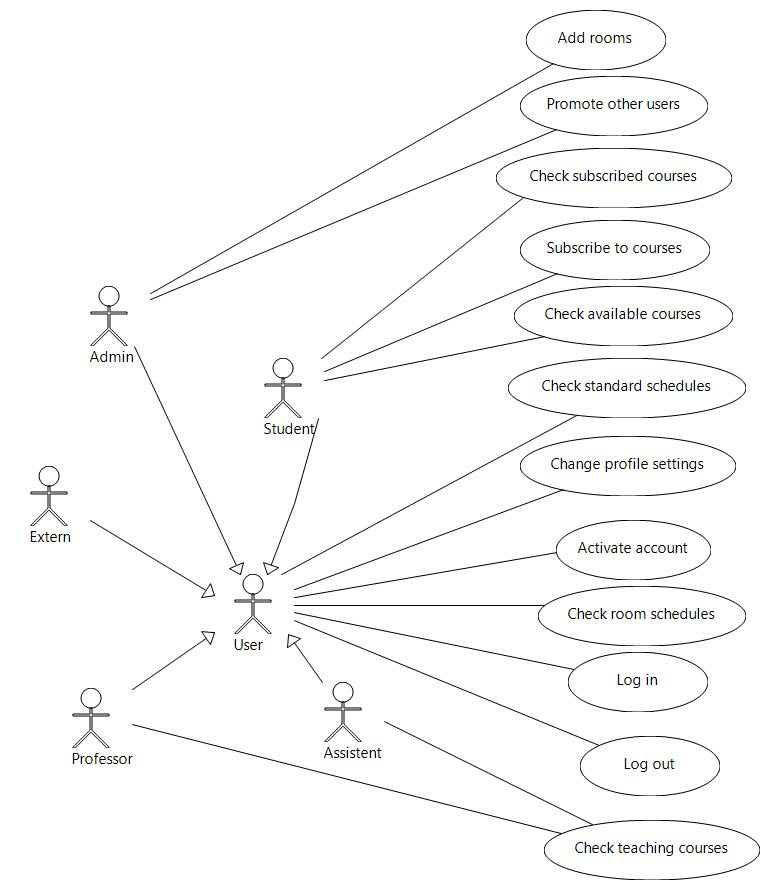
\includegraphics[scale=0.5]{design/papyrus/use_cases.jpg}
	\label{fig:usecase}
	\caption{Use case diagram}
	
\end{figure}

\section{Logica}
\label{sec:logica}
Uitleg implementatie en bestaande klassen.

\section{Data}
\label{sec:data}
DB schema met een woordje uitleg
